\chapter{Egyenletek}
\label{sec:Egyenletek}

\section{Tenzorszorzás azonosságai}

\definition[Asszociativitás]
\begin{align}
  (A \otimes B) \otimes C = A \otimes (B \otimes C)
\end{align}

\definition[Disztibutivitás a mátrixszorzás felett]
Ha A és C, illetve B és D kompatibilisek, akkor:
\begin{align}
  (A \otimes B)(C \otimes D) = (AC) \otimes (BD)
\end{align}


\definition[Lemma: Egységmátrixok beolvadása]
\begin{align}
  (A_n \otimes I_m)(I_n \otimes B_m) = A_n \otimes B_m
\end{align}


\section{Kvantumséta a rácson}

A következőkben a rácson, mint 4-reguláris gráfon vett bolyongást fogjuk
részletesen megvizsgálni.

Legyen a rács $N = n \times n$ -es.

Pozíció vektor: $\ket{P} =  (p_{0}, \dots, p_{N})$, ahol
$p_{i}\in\mathds{C}$ ahol $0 \leq{} i < N$, $\forall{}i$-re és $\sum\limits_{i=0}^{N} |p_i|^2 = 1$.

\begin{align}
  \ket{P_{0}} =  (0, \dots, 0, 1, 0, \dots, 0)
\end{align}

\begin{align}
  C = (\frac{1}{\sqrt{2}}, \frac{i}{\sqrt{2}}) \otimes (\frac{1}{\sqrt{2}}, \frac{i}{\sqrt{2}})
\end{align}

\begin{align}
  S_{\text{left}} =
  \begin{pmatrix}
    0      & 0      & 0      & \dots  & 0 \\
    1      & 0      & 0      & \dots  & 0 \\
    0      & 1      & 0      & \ddots & 0 \\
    \vdots & \ddots & \ddots & 0
  \end{pmatrix}
\end{align}

% https://hu.wikipedia.org/wiki/Kronecker_delta_f%C3%BCggv%C3%A9ny
\begin{definition}[Kronecker delta]
  Olyan kétváltozós függvény ami akkor $1$, ha a két változója egyenlő, egyébként $0$.
  \begin{align}
    \delta_{ij} =
    \begin{cases}
      0 & \text{ha $i\neq{}j$} \\
      1 & \text{ha $i=j$}
    \end{cases}
  \end{align}
\end{definition}

% https://en.wikipedia.org/wiki/Shift_matrix
\begin{definition}[Upper cyclic shift matrix]
  Az $U_{k}$ mátrix egy olyan ($k\times{}k$)-s mátrix, aminek a felső mellékátlóján és a bal alsó sarokban
  $1$-esek vannak, máshol $0$-k.
  Az index számozása moduló k történik.
  Ennek az $i$. sor, $j$. oszlopában:
  \begin{align}
    U_{k}[i,j] = \delta_{(i+1),j}
  \end{align}
\end{definition}

\begin{definition}[Lower cyclic shift matrix]
  Az $L_{k}$ mátrix egy olyan ($k\times{}k$)-s mátrix, aminek az alsó mellékátlóján és a jobb felső sarokban
  $1$-esek vannak, máshol $0$-k.
  Az index számozása moduló k történik.
  Ennek az $i$. sor, $j$. oszlopában:
  \begin{align}
    L_{k}[i,j] = \delta_{i,j+1}
  \end{align}
\end{definition}

\begin{align}
  L = U^{T}
\end{align}


\begin{itemize}
  \item Rács = két körnek a tenzorszorzata.
  \item Fel/le = mindig 1 sorral felette/alatta lévő (modulóval) van összekötve = n-el van elcsúsztatva.
  \item Függőlegesen számozva ugyanígy csak fordított elnevezések.
  \item Jobbra-balra = 1 távolság, kivéve sor végén, ahol a sor elejére ugrik = kis körök.
  \item Tenzorszorzás tulajdonságait előre kiszedni, műveletek, használatkor hivatkozni.
  \item Többsoros képleteknek csak 1 száma legyen.
\end{itemize}

\section{Példa}

\begin{align}
  n = 3
\end{align}

\begin{figure}[!ht]
  \begin{center}
    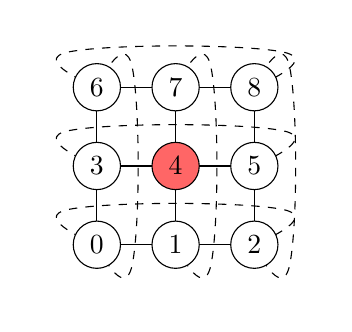
\begin{tikzpicture}

      \draw(0,0) -- (0,2);
      \draw(1,0) -- (1,2);
      \draw(2,0) -- (2,2);

      \draw [black, dashed] plot [smooth, tension=0.8] coordinates { (0,0) (0.45,-0.25) (0.45,2.25) (0,2)};
      \draw [black, dashed] plot [smooth, tension=0.8] coordinates { (1,0) (1.45,-0.25) (1.45,2.25) (1,2)};
      \draw [black, dashed] plot [smooth, tension=0.8] coordinates { (2,0) (2.45,-0.25) (2.45,2.25) (2,2)};


      \draw(0,0) -- (2,0);
      \draw(0,1) -- (2,1);
      \draw(0,2) -- (2,2);

      \draw [black, dashed] plot [smooth, tension=0.8] coordinates { (0,0) (-0.35,0.45) (2.35,0.45) (2,0)};
      \draw [black, dashed] plot [smooth, tension=0.8] coordinates { (0,1) (-0.35,1.45) (2.35,1.45) (2,1)};
      \draw [black, dashed] plot [smooth, tension=0.8] coordinates { (0,2) (-0.35,2.45) (2.35,2.45) (2,2)};

      \draw[black,fill=white](0,0) circle (0.3) node {0};
      \draw[black,fill=white](1,0) circle (0.3) node {1};
      \draw[black,fill=white](2,0) circle (0.3) node {2};

      \draw[black,fill=white](0,1) circle (0.3) node {3};
      \draw[black,fill=red!60](1,1) circle (0.3) node {4};
      \draw[black,fill=white](2,1) circle (0.3) node {5};

      \draw[black,fill=white](0,2) circle (0.3) node {6};
      \draw[black,fill=white](1,2) circle (0.3) node {7};
      \draw[black,fill=white](2,2) circle (0.3) node {8};

    \end{tikzpicture}
  \end{center}
  \caption{n=3-ös rács}
  \label{fig:3Racs}
\end{figure}

\begin{align}
  N = n^2 = 9
\end{align}

\begin{align}
  S_{\text{left}} = I_3 \otimes U_3 =
  \begin{pmatrix}
    0                  & \textcolor{red}{1} & 0                  & 0                  & 0                  & 0                  & 0                  & 0                  & 0                  \\
    0                  & 0                  & \textcolor{red}{1} & 0                  & 0                  & 0                  & 0                  & 0                  & 0                  \\
    \textcolor{red}{1} & 0                  & 0                  & 0                  & 0                  & 0                  & 0                  & 0                  & 0                  \\
    0                  & 0                  & 0                  & 0                  & \textcolor{red}{1} & 0                  & 0                  & 0                  & 0                  \\
    0                  & 0                  & 0                  & 0                  & 0                  & \textcolor{red}{1} & 0                  & 0                  & 0                  \\
    0                  & 0                  & 0                  & \textcolor{red}{1} & 0                  & 0                  & 0                  & 0                  & 0                  \\
    0                  & 0                  & 0                  & 0                  & 0                  & 0                  & 0                  & \textcolor{red}{1} & 0                  \\
    0                  & 0                  & 0                  & 0                  & 0                  & 0                  & 0                  & 0                  & \textcolor{red}{1} \\
    0                  & 0                  & 0                  & 0                  & 0                  & 0                  & \textcolor{red}{1} & 0                  & 0
  \end{pmatrix}
\end{align}

\begin{align}
  S_{\text{right}} = I_3 \otimes L_3 =
  \begin{pmatrix}
    0                  & 0                  & \textcolor{red}{1} & 0                  & 0                  & 0                  & 0                  & 0                  & 0                  \\
    \textcolor{red}{1} & 0                  & 0                  & 0                  & 0                  & 0                  & 0                  & 0                  & 0                  \\
    0                  & \textcolor{red}{1} & 0                  & 0                  & 0                  & 0                  & 0                  & 0                  & 0                  \\
    0                  & 0                  & 0                  & 0                  & 0                  & \textcolor{red}{1} & 0                  & 0                  & 0                  \\
    0                  & 0                  & 0                  & \textcolor{red}{1} & 0                  & 0                  & 0                  & 0                  & 0                  \\
    0                  & 0                  & 0                  & 0                  & \textcolor{red}{1} & 0                  & 0                  & 0                  & 0                  \\
    0                  & 0                  & 0                  & 0                  & 0                  & 0                  & 0                  & 0                  & \textcolor{red}{1} \\
    0                  & 0                  & 0                  & 0                  & 0                  & 0                  & \textcolor{red}{1} & 0                  & 0                  \\
    0                  & 0                  & 0                  & 0                  & 0                  & 0                  & 0                  & \textcolor{red}{1} & 0
  \end{pmatrix}
\end{align}


\begin{align}
  S_{\text{down}} = U_3^3 = U_3 \otimes I_3 =
  \begin{pmatrix}
    0                  & 0                  & 0                  & \textcolor{red}{1} & 0                  & 0                  & 0                  & 0                  & 0                  \\
    0                  & 0                  & 0                  & 0                  & \textcolor{red}{1} & 0                  & 0                  & 0                  & 0                  \\
    0                  & 0                  & 0                  & 0                  & 0                  & \textcolor{red}{1} & 0                  & 0                  & 0                  \\
    0                  & 0                  & 0                  & 0                  & 0                  & 0                  & \textcolor{red}{1} & 0                  & 0                  \\
    0                  & 0                  & 0                  & 0                  & 0                  & 0                  & 0                  & \textcolor{red}{1} & 0                  \\
    0                  & 0                  & 0                  & 0                  & 0                  & 0                  & 0                  & 0                  & \textcolor{red}{1} \\
    \textcolor{red}{1} & 0                  & 0                  & 0                  & 0                  & 0                  & 0                  & 0                  & 0                  \\
    0                  & \textcolor{red}{1} & 0                  & 0                  & 0                  & 0                  & 0                  & 0                  & 0                  \\
    0                  & 0                  & \textcolor{red}{1} & 0                  & 0                  & 0                  & 0                  & 0                  & 0
  \end{pmatrix}
\end{align}


\begin{align}
  S_{\text{up}} = L_3^3 = L_3 \otimes I_3 =
  \begin{pmatrix}
    0                  & 0                  & 0                  & 0                  & 0                  & 0                  & \textcolor{red}{1} & 0                  & 0                  \\
    0                  & 0                  & 0                  & 0                  & 0                  & 0                  & 0                  & \textcolor{red}{1} & 0                  \\
    0                  & 0                  & 0                  & 0                  & 0                  & 0                  & 0                  & 0                  & \textcolor{red}{1} \\
    \textcolor{red}{1} & 0                  & 0                  & 0                  & 0                  & 0                  & 0                  & 0                  & 0                  \\
    0                  & \textcolor{red}{1} & 0                  & 0                  & 0                  & 0                  & 0                  & 0                  & 0                  \\
    0                  & 0                  & \textcolor{red}{1} & 0                  & 0                  & 0                  & 0                  & 0                  & 0                  \\
    0                  & 0                  & 0                  & \textcolor{red}{1} & 0                  & 0                  & 0                  & 0                  & 0                  \\
    0                  & 0                  & 0                  & 0                  & \textcolor{red}{1} & 0                  & 0                  & 0                  & 0                  \\
    0                  & 0                  & 0                  & 0                  & 0                  & \textcolor{red}{1} & 0                  & 0                  & 0
  \end{pmatrix}
\end{align}

\begin{align}
  X_{\text{head}} =
  \begin{pmatrix}
    1 & 0 \\
    0 & 0
  \end{pmatrix}
\end{align}

\begin{align}
  X_{\text{tail}} =
  \begin{pmatrix}
    0 & 0 \\
    0 & 1
  \end{pmatrix}
\end{align}


\begin{align}
  S =
  (S_{\text{up}} S_{\text{left}}) \otimes (X_{\text{head}} \otimes X_{\text{head}}) +    \\
  (S_{\text{up}}  S_{\text{right}}) \otimes (X_{\text{head}} \otimes X_{\text{tail}}) +  \\
  (S_{\text{down}}  S_{\text{left}}) \otimes (X_{\text{tail}} \otimes X_{\text{head}}) + \\
  (S_{\text{down}} S_{\text{right}}) \otimes (X_{\text{tail}} \otimes X_{\text{tail}})
\end{align}

\begin{align}
  C_4 = H^{\otimes2} = \frac{1}{2}
  \begin{pmatrix}
    1 & 1  & 1  & 1  \\
    1 & -1 & 1  & -1 \\
    1 & 1  & -1 & -1 \\
    1 & -1 & -1 & 1
  \end{pmatrix}
\end{align}

\begin{align}
  U = S  (I_9 \otimes C_4)
\end{align}

\begin{align}
  U =
  ((S_{\text{up}}  S_{\text{left}}) \otimes (X_{\text{head}} \otimes X_{\text{head}}) +  \\
  (S_{\text{up}} S_{\text{right}}) \otimes (X_{\text{head}} \otimes X_{\text{tail}}) +   \\
  (S_{\text{down}}  S_{\text{left}}) \otimes (X_{\text{tail}} \otimes X_{\text{head}}) + \\
  (S_{\text{down}} S_{\text{right}}) \otimes (X_{\text{tail}} \otimes X_{\text{tail}}))
  (I_9 \otimes C_4)
\end{align}

\definition[Tenzorszorzás azonosság: mátrix szorzással disztibutív]

Bal oldalt 9*9-es, jobb oldalt 4*4-es mátrixok vannak.

\begin{align}
  U =
  (S_{\text{up}}  S_{\text{left}}) \otimes ((X_{\text{head}} \otimes X_{\text{head}})  C_4) +   \\
  (S_{\text{up}}  S_{\text{right}}) \otimes ((X_{\text{head}} \otimes X_{\text{tail}}) C_4) +   \\
  (S_{\text{down}}  S_{\text{left}}) \otimes ((X_{\text{tail}} \otimes X_{\text{head}})  C_4) + \\
  (S_{\text{down}}  S_{\text{right}}) \otimes ((X_{\text{tail}} \otimes X_{\text{tail}}) C_4)
\end{align}

\begin{align}
  C_4 = C_2 \otimes C_2
\end{align}

\begin{align}
  U =
  (S_{\text{up}}  S_{\text{left}}) \otimes ((X_{\text{head}} \otimes X_{\text{head}}) (C_2 \otimes C_2)) +   \\
  (S_{\text{up}}  S_{\text{right}}) \otimes ((X_{\text{head}} \otimes X_{\text{tail}}) (C_2 \otimes C_2)) +  \\
  (S_{\text{down}}  S_{\text{left}}) \otimes ((X_{\text{tail}} \otimes X_{\text{head}}) (C_2 \otimes C_2)) + \\
  (S_{\text{down}}  S_{\text{right}}) \otimes ((X_{\text{tail}} \otimes X_{\text{tail}}) (C_2 \otimes C_2))
\end{align}

\definition[Tenzorszorzás azonosság: mátrix szorzással disztibutív]

\begin{align}
  U =
  (S_{\text{up}}  S_{\text{left}}) \otimes (((X_{\text{head}}C_2) \otimes (X_{\text{head}}C_2))) +   \\
  (S_{\text{up}}  S_{\text{right}}) \otimes (((X_{\text{head}}C_2) \otimes (X_{\text{tail}}C_2))) +  \\
  (S_{\text{down}}  S_{\text{left}}) \otimes (((X_{\text{tail}}C_2) \otimes (X_{\text{head}}C_2))) + \\
  (S_{\text{down}}  S_{\text{right}}) \otimes (((X_{\text{tail}}C_2) \otimes (X_{\text{tail}}C_2)))
\end{align}

\definition[Tenzorszorzás azonosság: asszociatív]


\begin{align}
  U =
  (S_{\text{up}}  S_{\text{left}}) \otimes (X_{\text{head}}C_2) \otimes (X_{\text{head}}C_2) +   \\
  (S_{\text{up}}  S_{\text{right}}) \otimes (X_{\text{head}}C_2) \otimes (X_{\text{tail}}C_2) +  \\
  (S_{\text{down}}  S_{\text{left}}) \otimes (X_{\text{tail}}C_2) \otimes (X_{\text{head}}C_2) + \\
  (S_{\text{down}}  S_{\text{right}}) \otimes (X_{\text{tail}}C_2) \otimes (X_{\text{tail}}C_2)
\end{align}


\definition[Tenzorszorzás Lemma?]


\begin{align}
  S = ((S_{\text{up}} \otimes  X_{\text{head}} \otimes I) +
  (S_{\text{down}} \otimes X_{\text{tail}} \otimes I))
  ((S_{\text{left}} \otimes I \otimes X_{\text{head}}) +
  (S_{\text{right}} \otimes I \otimes  X_{\text{tail}} ))
\end{align}


% \begin{align}
%   U =
%   ((S_{\text{up}}  S_{\text{left}}) \otimes I_2) (I_9 \otimes (X_{\text{head}}C_2)) \otimes (X_{\text{head}}C_2) +   \\
%   ((S_{\text{up}}  S_{\text{right}}) \otimes I_2) (I_9 \otimes (X_{\text{head}}C_2)) \otimes (X_{\text{tail}}C_2) +  \\
%   ((S_{\text{down}}  S_{\text{left}}) \otimes I_2) (I_9 \otimes (X_{\text{tail}}C_2)) \otimes (X_{\text{head}}C_2) + \\
%   ((S_{\text{down}}  S_{\text{right}}) \otimes I_2) (I_9 \otimes (X_{\text{tail}}C_2)) \otimes (X_{\text{tail}}C_2)
% \end{align}